\documentclass[notes]{beamer}
\usetheme{Madrid}
\usecolortheme{whale}

\definecolor{darkgreen}{rgb}{0.0, 0.2, 0.13}
\definecolor{burntorange}{rgb}{0.8, 0.33, 0.0}
\definecolor{darkmidnightblue}{rgb}{0.0, 0.2, 0.4}
\definecolor{darkslateblue}{rgb}{0.28, 0.24, 0.55}

% Logo and footer setup
\usepackage{graphicx}
\usepackage{tikz}
\usetikzlibrary{positioning, arrows}

% Custom footer
\setbeamertemplate{footline}{
  \leavevmode%
  \hbox{%
  \begin{beamercolorbox}[wd=.1\paperwidth,ht=2.25ex,dp=1ex,center]{date in head/foot}%
    
\includegraphics[height=2ex]{ua_logo.png}
  \end{beamercolorbox}%
  \begin{beamercolorbox}[wd=.8\paperwidth,ht=2.25ex,dp=1ex,center]{title in head/foot}%
    \usebeamerfont{title in head/foot}\insertshorttitle
  \end{beamercolorbox}%
  \begin{beamercolorbox}[wd=.1\paperwidth,ht=2.25ex,dp=1ex,right]{date in head/foot}%
    \usebeamerfont{date in head/foot}\insertframenumber{}/\inserttotalframenumber\hspace*{2ex}
  \end{beamercolorbox}}%
  \vskip0pt%
}

\title{Document Clustering System with Docker}
\subtitle{Technical Mathematics for Big Data}
\author{Oyedotun Oluwasegun Michael (\#123168) \\ Silvia Mastracci (\#123177) \\ Oleksandr Solovei (\#126784)}
\date{January 16, 2025}

\begin{document}

\begin{frame}
    \titlepage
\end{frame}

{
\setbeamercolor{frametitle}{bg=darkmidnightblue}
\begin{frame}{Project Overview}
  \begin{columns}[T] % 'T' aligns columns at the top
    \begin{column}{0.34\textwidth}
    \begin{itemize}
        \item Document Clustering System built with microservices
        \item Containerized solution using Docker technology
        \vspace{.5cm}
        \item React-based UI
        \item Flask microservices
        \item Elasticsearch engine
        \item Document analysis system
    \end{itemize}
    \end{column}
    \begin{column}{0.62\textwidth}
    % https://mermaid.ink/img/pako:eNp9VMFu2zAM_RVBvayACmwr0HU-DNgWF-ihQxFvPczJQZWo2IgtBZKctij676MkO3ZWIzpYFPlIPoqUX6kwEmhGVWOeRMWtJ78XK01w_XFgy59NDdqTH9Y84XFNLi6-kV-bWj-X8UuWsAfrgNxb8_yyTo7p67rHjeW7iiyM2IIlud7X1ugWwyVAWClICHqDNg9alkvgwh-OpAC7rwWs53y-39-WNw132yCdRBbArajKtJ1EIlusRZS4d4FrqEyAc8ZO4KMUEo8J3uv7cHOuPZmAyosyxzp8LVxUrmdRS5C1Gy196DnTKOVFn-DBNOWHoyQEVVji-SRZDDMGjD5J9x47TY9yxB4u7RiOfZxOhkAWbgGKuNQHouqmyc74NVwJxZy3ZgvZ2eXj1dcv1_957MKY9XilJGJO4503lm-GDFKAFJ9Oe-wj80MK9Zl_nHWYuMWXwvonQiQo3jV-ak_TFblP1cOMMxwWlvrMhlvtr2YKzwuWetEXdWzDG2dD01jqR18LZbQF2_Ja4jN_DV4r6itoYUUzFAe-dKXfEMo7b4oXLWjmbQeMWtNtKpop3jg8dTvJPSxqjk-7PWh3XP81ZjwjDaR4l34s8f_y9g_PU2Kj?type=png)](https://mermaid.live/edit#pako:eNp9VMFu2zAM_RVBvayACmwr0HU-DNgWF-ihQxFvPczJQZWo2IgtBZKctij676MkO3ZWIzpYFPlIPoqUX6kwEmhGVWOeRMWtJ78XK01w_XFgy59NDdqTH9Y84XFNLi6-kV-bWj-X8UuWsAfrgNxb8_yyTo7p67rHjeW7iiyM2IIlud7X1ugWwyVAWClICHqDNg9alkvgwh-OpAC7rwWs53y-39-WNw132yCdRBbArajKtJ1EIlusRZS4d4FrqEyAc8ZO4KMUEo8J3uv7cHOuPZmAyosyxzp8LVxUrmdRS5C1Gy196DnTKOVFn-DBNOWHoyQEVVji-SRZDDMGjD5J9x47TY9yxB4u7RiOfZxOhkAWbgGKuNQHouqmyc74NVwJxZy3ZgvZ2eXj1dcv1_957MKY9XilJGJO4503lm-GDFKAFJ9Oe-wj80MK9Zl_nHWYuMWXwvonQiQo3jV-ak_TFblP1cOMMxwWlvrMhlvtr2YKzwuWetEXdWzDG2dD01jqR18LZbQF2_Ja4jN_DV4r6itoYUUzFAe-dKXfEMo7b4oXLWjmbQeMWtNtKpop3jg8dTvJPSxqjk-7PWh3XP81ZjwjDaR4l34s8f_y9g_PU2Kj
        \centering  % Center the image horizontally
        \vspace{0.5cm}  % Adjust top margin
        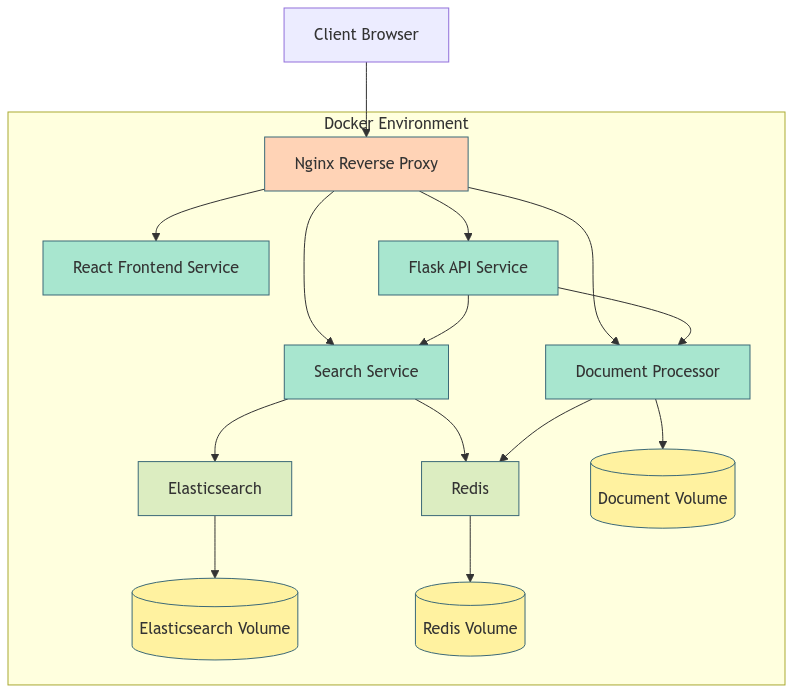
\includegraphics[width=0.95\textwidth,height=0.7\textheight,keepaspectratio]{systemarch.png}
    \end{column}
  \end{columns}
\end{frame}

\begin{frame}[fragile]{Docker Setup and Operations}
  \begin{columns}[T] % 'T' aligns columns at the top
    \begin{column}{0.48\textwidth} % Slightly reduced width for margin
      \begin{beamercolorbox}[shadow=true,rounded=true]{block title}
        \centering\textbf{Docker Compose Config}
      \end{beamercolorbox}
        \begin{verbatim}
services:
  nginx:
    image: nginx:alpine
    ports:
      - "4321:80"
  frontend:
    build: ./frontend
    expose:
      - "3000"
  api:
    build: ./api
    expose:
      - "8000"
  document-processor: (...)
  search: (...)
        \end{verbatim}
    \end{column}
    
    \hspace{0.5em} % Add horizontal space between columns
    
    \begin{column}{0.48\textwidth}
      \begin{beamercolorbox}[shadow=true,rounded=true]{block title}
        \centering\textbf{Common Commands}
      \end{beamercolorbox}

        \begin{verbatim}
# Build and start
docker-compose up --build

# Stop services
docker-compose down

# View logs
docker-compose logs -f

# Rebuild specific service
docker-compose build svc-name

# Show running containers
docker-compose ps
        \end{verbatim}
    \end{column}
  \end{columns}
\end{frame}

\begin{frame}{Docker Benefits}
  \begin{columns}[T]
    \begin{column}{0.32\textwidth}
        \begin{beamercolorbox}[shadow=true,rounded=true]{block title}
        \centering 
        
\includegraphics[width=0.4\textwidth]{coding.png}\\[0.3em]
        For Development
      \end{beamercolorbox}
      \begin{itemize}
        \item \textbf{Consistent Environment} \\[-0.4em]
        {\tiny no "works on my machine"}
        \item \textbf{Isolated Deps} \\[-0.4em]
        {\tiny no version conflicts}
        \item \textbf{Rapid Dev Cycle} \\[-0.4em]
        {\tiny fast startup, easy rollbacks}
      \end{itemize}
    \end{column}
    
    \hspace{0.2em}
    
    \begin{column}{0.32\textwidth}
\begin{beamercolorbox}[shadow=true,rounded=true]{block title}
        \centering 
        
\includegraphics[width=0.4\textwidth]{performance.png}\\[0.3em]
        For Performance
      \end{beamercolorbox}
      \begin{itemize}
        \item \textbf{Resource Efficiency} \\[-0.4em]
        {\tiny lightweight architecture}
        \item \textbf{Scalability} \\[-0.4em]
        {\tiny horizontal scaling}
        \item \textbf{Maintenance} \\[-0.4em]
        {\tiny simple updates, min downtime}
      \end{itemize}
    \end{column}
    
    \hspace{0.2em}
    
    \begin{column}{0.32\textwidth}
\begin{beamercolorbox}[shadow=true,rounded=true]{block title}
        \centering 
        
\includegraphics[width=0.4\textwidth]{security.png}\\[0.3em]
        For Security
      \end{beamercolorbox}
      \begin{itemize}
        \item \textbf{Vulnerability Management} \\[-0.4em]
        {\tiny image scanning, regular updates}
        \item \textbf{Instance Isolation} \\[-0.4em]
        {\tiny for processes and networks}
        \item \textbf{Security Features} \\[-0.4em]
        {\tiny access \& resource limits}
      \end{itemize}
    \end{column}
  \end{columns}
\end{frame}
}

{
\setbeamercolor{frametitle}{bg=darkgreen}
\begin{frame}{Core Components of Docker}
    \textbf{Docker Client \& Server (Engine)}: The client sends commands to the server (Docker Engine), which builds, runs, and manages containers. \\
    
    \textbf{Docker Images}: A Docker image is a blueprint for creating containers, built using a Dockerfile. \\
    
    \textbf{Docker Containers}: A Docker container is a running instance of a Docker image, providing isolated environments for applications. \\
    
    \textbf{Docker Registries}: A Docker registry stores and distributes Docker images. Examples include Docker Hub and private registries. \\
\end{frame}
\begin{frame}[fragile]{Using Docker for Clustering }
\textbf{structure}

\begin{verbatim}
clustering-project/
├── app/   # Source code for both document and image clustering
│   ├── document_clustering/    # Document clustering code
│   │   ├── main.py          # Entry point for document clustering
│   │   ├── clustering.py  # Core clustering logic (e.g., K-means)
│   │   ├── utils.py      # Text preprocessing (tokenization, etc)
│   │   └── requirements.txt    # Document clustering dependencies 
│   ├── image_clustering/       # Image clustering code
│   │   ├── main.py          # Entry point for image clustering
│   │   ├── clustering.py  # Core clustering logic (e.g., DBSCAN)
│   │   ├── utils.py        # Image preprocessing (resizing, CNN)
│   │   └── requirements.txt  # Image clustering dependencies (tensorflow)
├── data/                       # Stores input and output files
│   ├── documents/              # Raw text documents
│   ├── images/                 # Raw image files

\end{verbatim}
\end{frame}

\begin{frame}[fragile]{Using Docker for Clustering }
\begin{verbatim}
│   └── processed/  # Processed output (clusters, visualizations)
├── Dockerfile   # Configuration for containerization
├── docker-compose.yml  # Multi-container setup for both clustering apps
├── README.md                   # Project documentation
└── requirements.txt   # Common dependencies (e.g.,numpy,pandas)
\end{verbatim} 


 \begin{itemize}
        \item \textbf{`app/`}: Contains source code for both tasks:
        \begin{itemize}
            \item \textbf{`document clustering/`}: Includes Python scripts like \texttt{main.py}, \texttt{clustering.py} (e.g., K-means), and \texttt{utils.py} (text preprocessing). Dependencies include \texttt{scikit-learn}, \texttt{nltk}, and \texttt{spaCy}.
            \item \textbf{`image clustering/`}: Includes scripts like \texttt{main.py}, \texttt{clustering.py}, and \texttt{utils.py} (image preprocessing). Dependencies include \texttt{opencv}, \texttt{PIL}, and \texttt{tensorflow}.
        \end{itemize}
        
        \item \textbf{`data/`}: Stores input and output data:
        \begin{itemize}
            \item \textbf{`documents/`}, \textbf{`images/`} (raw files) and \textbf{`processed/`} (output from clustering).
        \end{itemize}
    \end{itemize}  
\end{frame}

\begin{frame}{Dockerfile Components for Document and Image Clustering}
    \begin{itemize}
        \item \textbf{Base Image}: \\
        \texttt{FROM python:3.8-slim} \\
        A lightweight Python image to start from for both document and image clustering.
        
        \item \textbf{Working Directory}: \\
        \texttt{WORKDIR /app} \\
        Defines the working directory inside the container.
        
        \item \textbf{Copy Application Files}: \\
        \texttt{COPY . /app} \\
        Copies project files (document\_clustering/ or image\_clustering/) into the container.
        
        \item \textbf{Install Dependencies}: \\
        \texttt{RUN pip install -r requirements.txt} \\
       
   \end{itemize}
\end{frame}
        
        \begin{frame}{Dockerfile Components for Document and Image Clustering}
    
        Installs necessary dependencies for the respective clustering task (e.g., \texttt{scikit-learn} for document clustering or \texttt{opencv}, \texttt{tensorflow} for image clustering).
        \begin{itemize}
        \item \textbf{Expose Ports (Optional)}: \\
        \texttt{EXPOSE 8000} \\
        If exposing a web app or API, define the port to be accessed outside the container.
        
        \item \textbf{Run the Application}: \\
        \textbf{Document Clustering}: \texttt{CMD ["python", "document\_clustering/main.py"]} \\
        \textbf{Image Clustering}: \texttt{CMD ["python", "image\_clustering/main.py"]} \\
        Executes the clustering application when the container starts.
    \end{itemize}
\end{frame}


}

{
\setbeamercolor{frametitle}{bg=darkmidnightblue}
\begin{frame}[fragile]{Project Implementation and System Features}
    % Use T (top baseline) alignment for columns themselves
    \begin{columns}[T]
        % Left column with text
        \begin{column}{0.48\textwidth}
            \begin{itemize}
                \item \textbf{Multi-stage builds}
                \begin{itemize}\small
                    \item Optimized image sizes
                    \item Reduced attack surface
                \end{itemize}

                \vspace{0.2cm}
                
                \item \textbf{Docker Compose}
                \begin{itemize}\small
                    \item Service orchestration
                    \item Environment configuration
                    \item Network management
                \end{itemize}

                \vspace{0.2cm}
                
                \item \textbf{Volume Management}
                \begin{itemize}\small
                    \item Persistent data storage
                    \item Efficient data sharing
                \end{itemize}
                
            \end{itemize}

            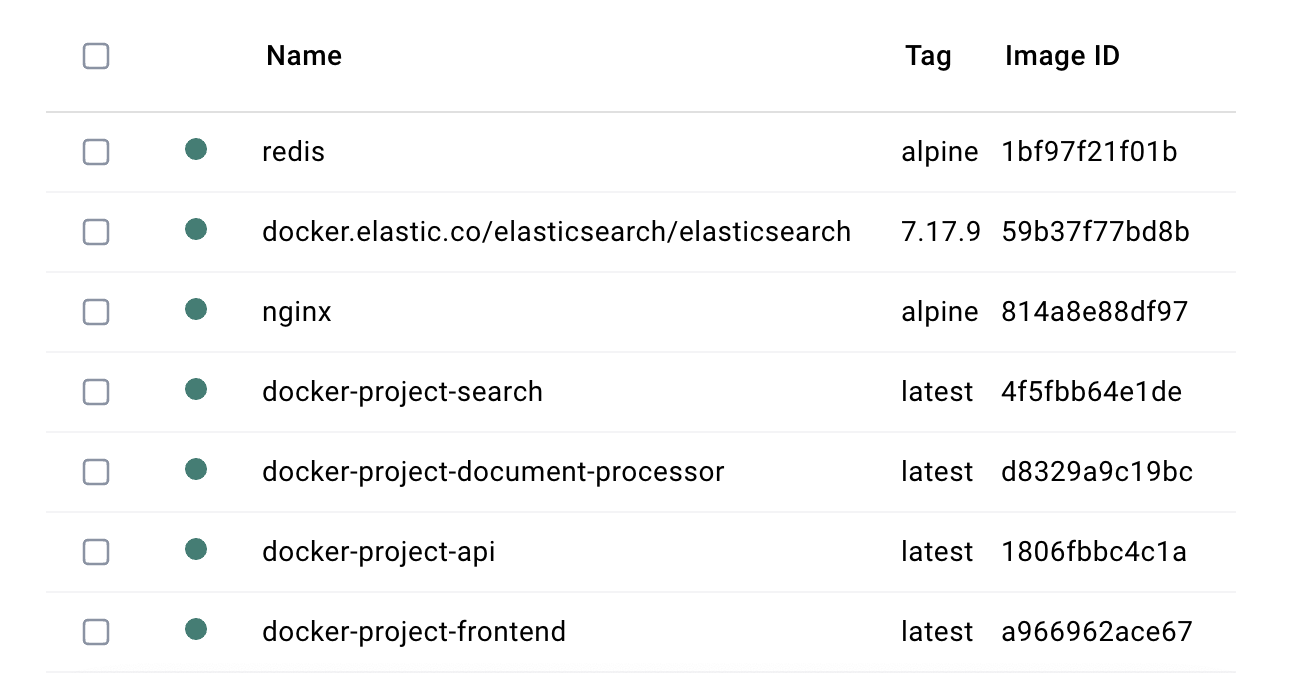
\includegraphics[width=0.95\textwidth,height=0.7\textheight,keepaspectratio]{docker_screenshot.png}
        \end{column}
        
        % Right column with image
        \begin{column}{0.48\textwidth}
            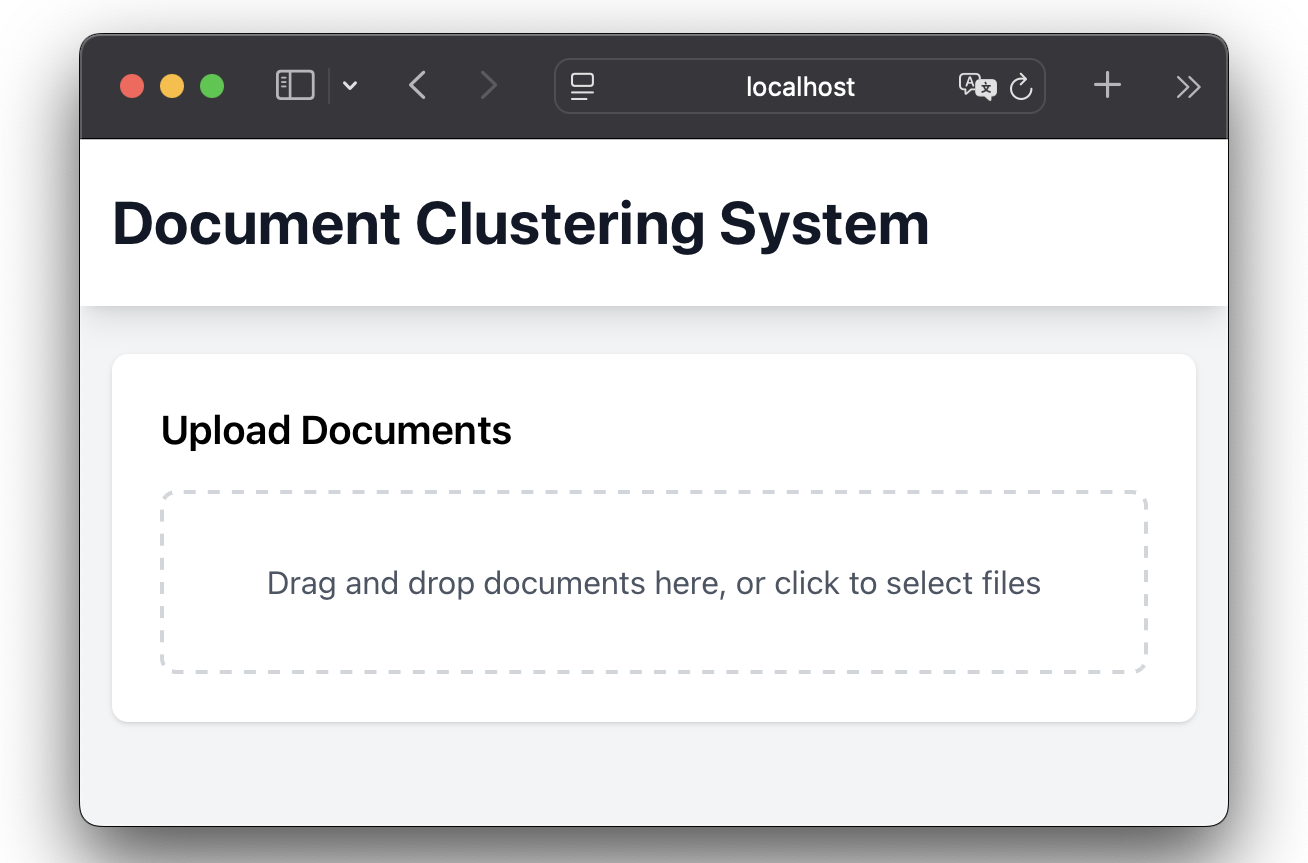
\includegraphics[width=0.9\textwidth,height=0.7\textheight,keepaspectratio]{app_screenshot.png}

            \begin{itemize}
                \item \textbf{Single Port Access}
                \begin{itemize}
                    \item All services through one port
                    \item Nginx reverse proxy
                    %\item Simplified deployment
                \end{itemize}
                \item \textbf{Monitoring}
                \begin{itemize}
                    \item Health checks
                    %\item Service discovery
                    \item Automated recovery
                \end{itemize}
                \item \textbf{Data Management}
                \begin{itemize}
                    \item Elasticsearch integration
                    \item Redis caching
                    \item Persistent storage
                \end{itemize}
            \end{itemize}
        \end{column}
    \end{columns}
\end{frame}
}

{
\setbeamercolor{frametitle}{bg=darkslateblue}

\begin{frame}{Performance Optimization with Parallelization}
    %\textbf{Parallel Document Processing}
    %\begin{itemize}
        %\item Use \texttt{ThreadPoolExecutor} to process multiple documents in parallel:
        %\begin{itemize}
            %\item OCR: Split documents into pages for concurrent processing.
            %\item Translations: Batch requests for multiple documents.
        %\end{itemize}
        %\item Redis caches embeddings to avoid reprocessing.
    %\end{itemize}
    \textbf{Document Processing Flowchart}
    \begin{center}
        \resizebox{0.75\textwidth}{!}{ % Adjusted size for better layout
            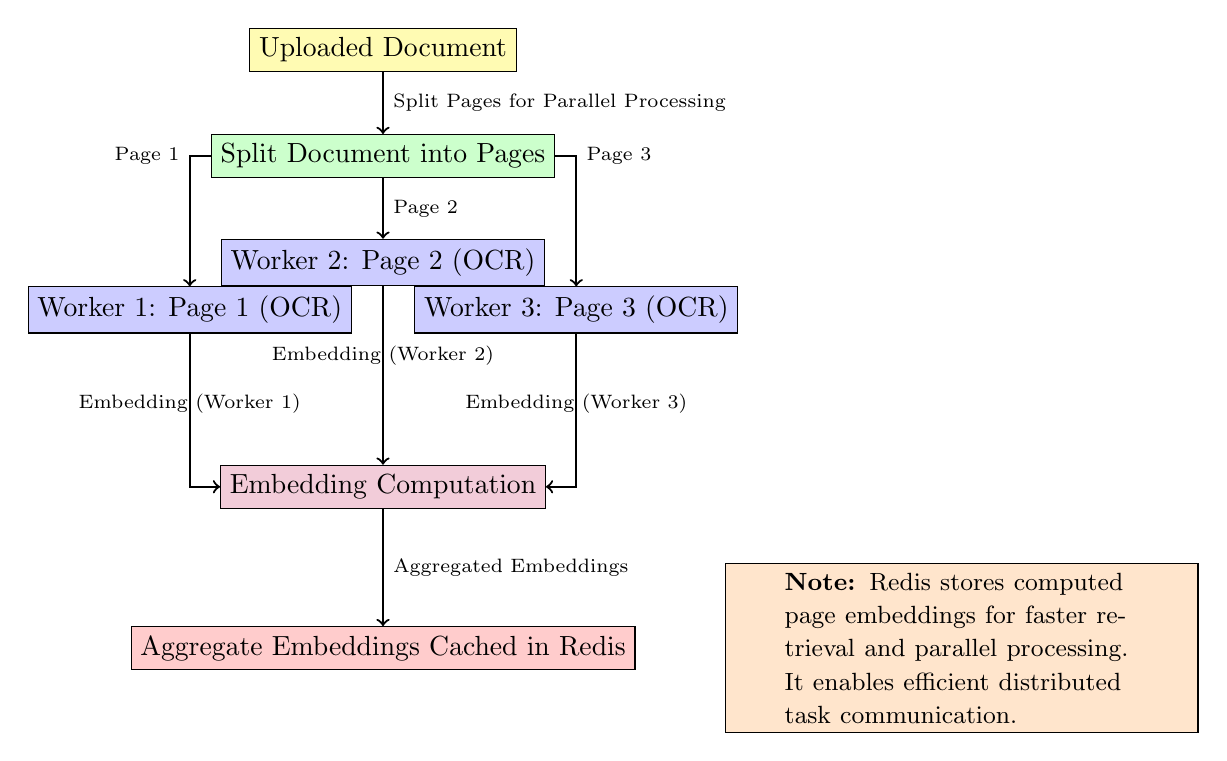
\begin{tikzpicture}[node distance=1.35cm, auto]
            % Nodes
            \node (input) [rectangle, draw, fill=yellow!30, minimum width=2cm] {Uploaded Document};
            \node (split) [rectangle, draw, fill=green!20, below of=input, minimum width=3cm] {Split Document into Pages};
            \node (worker1) [rectangle, draw, fill=blue!20, below left of=split, xshift=-1.5cm, yshift=-1cm] {Worker 1: Page 1 (OCR)};
            \node (worker2) [rectangle, draw, fill=blue!20, below of=split] {Worker 2: Page 2 (OCR)};
            \node (worker3) [rectangle, draw, fill=blue!20, below right of=split, xshift=1.5cm, yshift=-1cm] {Worker 3: Page 3 (OCR)};
            \node (embeddingNode) [rectangle, draw, fill=purple!20, below of=worker2, yshift=-1.5cm, minimum width=3cm] {Embedding Computation};
            \node (output) [rectangle, draw, fill=red!20, below of=embeddingNode, yshift=-0.7cm, minimum width=3cm] {Aggregate Embeddings Cached in Redis};
        
            % Arrows
            \draw[->, thick] (input) -- (split) node[midway, right] {\scriptsize Split Pages for Parallel Processing};
            \draw[->, thick] (split) -| (worker1) node[midway, left] {\scriptsize Page 1};
            \draw[->, thick] (split) -- (worker2) node[midway, right] {\scriptsize Page 2};
            \draw[->, thick] (split) -| (worker3) node[midway, right] {\scriptsize Page 3};
            \draw[->, thick] (worker1) |- (embeddingNode) node[midway, above=0.8] {\scriptsize Embedding (Worker 1)};
            \draw[->, thick] (worker2) -- (embeddingNode) node[midway, above] {\scriptsize Embedding (Worker 2)};
            \draw[->, thick] (worker3) |- (embeddingNode) node[midway, above=0.8] {\scriptsize Embedding (Worker 3)};
            \draw[->, thick] (embeddingNode) -- (output) node[midway, right] {\scriptsize Aggregated Embeddings};
        

        
            % Note about caching
            \node (note) [rectangle, draw, fill=orange!20, right of=output, xshift=6cm, minimum width=6cm, text width=4.5cm, align=left] {\small \textbf{Note:} Redis stores computed page embeddings for faster retrieval and parallel processing.
            It enables efficient distributed task communication.};

            \end{tikzpicture}
        }

    \end{center}


    \textbf{Future Enhancements}
    \begin{itemize}
        \item Implement \texttt{Celery} + Redis for distributed task queues.
        \item Add more workers to scale up parallel computations.
    \end{itemize}
\end{frame}

% Slide 4: Cloud Deployment & Blue-Green Strategy
\begin{frame}{Cloud Deployment \& Blue-Green Strategy}
            %\textbf{Blue-Green Deployment Flowchart}
            \resizebox{1.0\textwidth}{!}{
            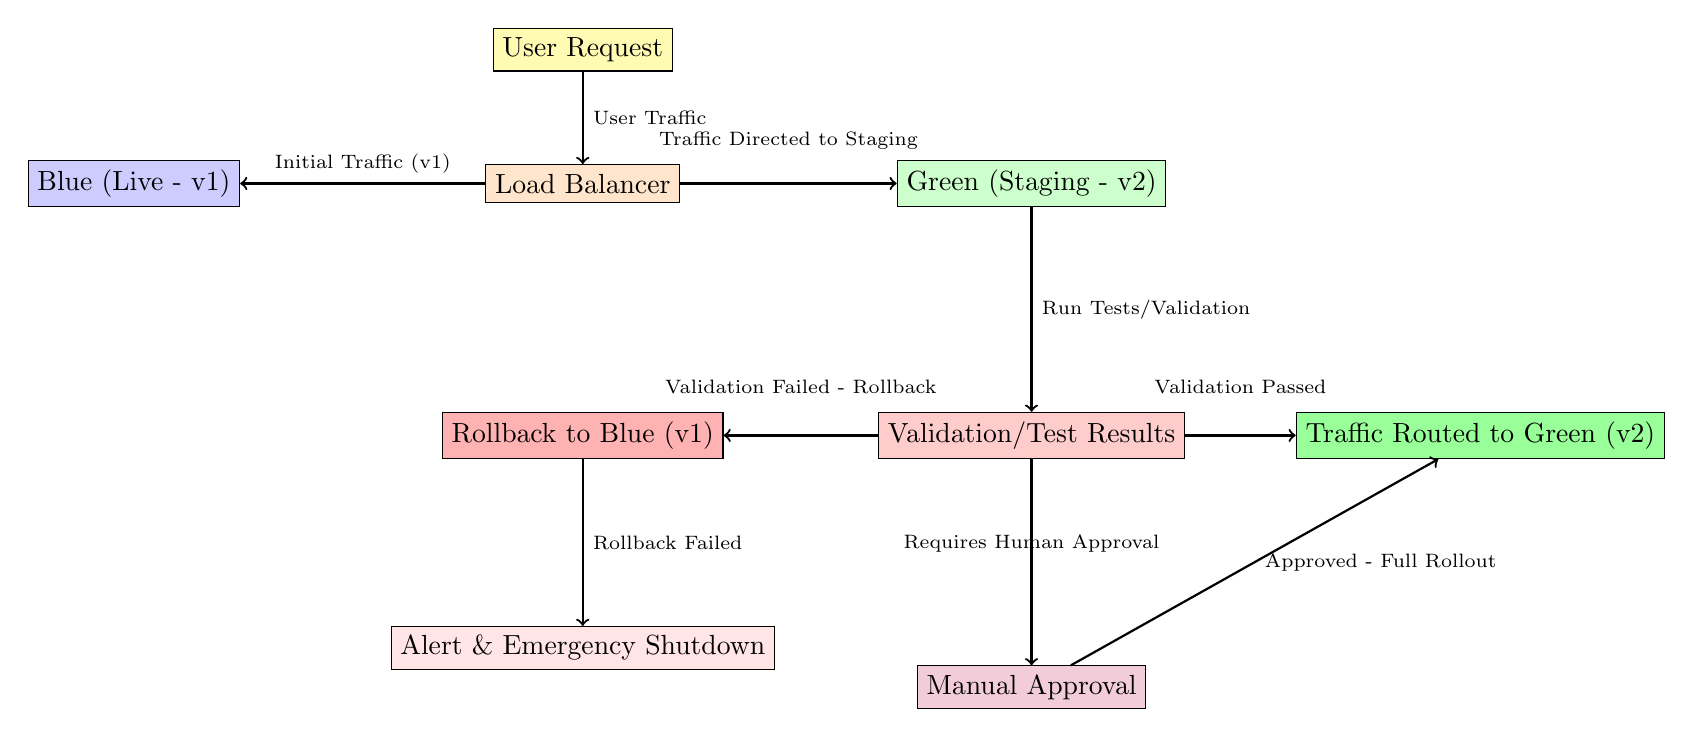
\begin{tikzpicture}[node distance=1.7cm, auto]
            % Nodes
            \node (user) [rectangle, draw, fill=yellow!30] {User Request};
            \node (lb) [rectangle, draw, fill=orange!20, below of=user] {Load Balancer};
            \node (blue) [rectangle, draw, fill=blue!20, left of=lb, xshift=-4cm] {Blue (Live - v1)};
            \node (green) [rectangle, draw, fill=green!20, right of=lb, xshift=4cm] {Green (Staging - v2)};
            \node (validation) [rectangle, draw, fill=red!20, below of=green, yshift=-1.5cm] {Validation/Test Results};
            \node (approval) [rectangle, draw, fill=purple!20, below of=validation, yshift=-1.5cm] {Manual Approval};
            \node (trafficGreen) [rectangle, draw, fill=green!40, right of=validation, xshift=4cm] {Traffic Routed to Green (v2)};
            \node (rollback) [rectangle, draw, fill=red!30, left of=validation, xshift=-4cm] {Rollback to Blue (v1)};
            \node (alert) [rectangle, draw, fill=red!10, below of=rollback, yshift=-1cm] {Alert \& Emergency Shutdown};
        
            % Arrows
            \draw[->, thick] (user) -- (lb) node[midway] {\scriptsize User Traffic};
            \draw[->, thick] (lb) -- (blue) node[midway, above] {\scriptsize Initial Traffic (v1)};
            \draw[->, thick] (lb) -- (green) node[midway, above=0.3] {\scriptsize Traffic Directed to Staging};
            \draw[->, thick] (green) -- (validation) node[midway, right] {\scriptsize Run Tests/Validation};
            \draw[->, thick] (validation) -- (trafficGreen) node[midway, above=0.4] {\scriptsize Validation Passed};
            \draw[->, thick] (validation) -- (approval) node[midway, above] {\scriptsize Requires Human Approval};
            \draw[->, thick] (validation) -- (rollback) node[midway, above=0.4] {\scriptsize Validation Failed - Rollback};
            \draw[->, thick] (rollback) -- (alert) node[midway, right] {\scriptsize Rollback Failed};
            \draw[->, thick] (approval) -- (trafficGreen) node[midway, right] {\scriptsize Approved - Full Rollout};
            \end{tikzpicture}


            }\\
            \textbf{Key Benefits:}
            \begin{itemize}
                \item Zero-downtime upgrades.
                \item Easy rollback if staging fails.
                \item Safer deployments with validation.
            \end{itemize}
            
\end{frame}

\begin{frame}{Cloud Development & Blue-Green Strategy}
    \textbf{Cloud Platforms:}
            \begin{itemize}
                \item AWS ECS/EKS: Docker container orchestration.
                \item Azure AKS: Managed Kubernetes clusters.
                \item DigitalOcean App Platform: Simplified deployments.
            \end{itemize}
    \vspace{0.05cm}
    
    \textbf{Next Steps:}
    \begin{itemize}
        \item Test load balancer configuration locally with Nginx.
    \end{itemize}
\end{frame}


% Slide 5: Migration to Kubernetes
\begin{frame}{Migration to Kubernetes}

\begin{columns}[T]
    \begin{column}{0.5\textwidth}
        \textbf{Why Kubernetes?}
        \begin{itemize}
            \item Self-healing, auto-scaling, and automated rollouts.
            \item Handles complex deployments with better orchestration.
        \end{itemize}
    \end{column}
        \vspace{0.5cm}
    \begin{column}{0.5\textwidth}
        \textbf{Migration Plan}
        \begin{itemize}
            \item Convert \texttt{docker-compose.yml} to Kubernetes manifests using:
            \begin{scriptsize}
            \texttt{kubectl apply -f deployment.yml}
            \end{scriptsize}
            \item Use Helm charts for templating reusable manifests.
        \end{itemize}
    \end{column}
\end{columns}

\vspace{0.4cm}

\textbf{Key Kubernetes Components:}
\begin{center}
    \begin{tabular}{|p{3cm}|p{6cm}|}
        \hline
        \textbf{Component} & \textbf{Purpose} \\ \hline
        \textbf{Pods}       & Smallest deployable unit containing containers. \\ \hline
        \textbf{Deployments} & Manage replica sets of pods to ensure availability and updates. \\ \hline
        \textbf{Services}   & Expose pods to external traffic and other components. \\ \hline
    \end{tabular}
\end{center}
\end{frame}
}

\begin{frame}{Conclusion}
    \begin{center}
        \Large{Thank You}
        
        \vspace{0.5cm}
        \normalsize{Document Clustering System}\\
        Docker-based Microservices Architecture
        
        \vspace{0.5cm}
        Questions?
    \end{center}
\end{frame}


\end{document}